\section{Analyse univariée}

\begin{frame}
	Prédiction et évaluation des risques
	\begin{itemize}
		\item Connaissances à transférer à la machine apprenante
		\begin{itemize}
			\item Prédire le risque relatif d'une sitation étant donnée certains précurseurs
		\end{itemize}	
		
		\item Éléments à modéliser
		\begin{itemize}
			\item fonction de densité des risques associés à la construction
		\end{itemize}	
	\end{itemize}
\end{frame}


\begin{frame}
	\begin{itemize}
	\item Données entrantes
	\begin{itemize}
		\item Banque de données de 921 rapport avec évaluation des sévérités par Esmaeili and Hallowell. Seuls 814 ont été conservés.
		\item La sévérité est sous-divisée en 5 classes.
		\item Extraction des précurseurs de risques de ces rapports avec l'outil développé plus tôt.
		\end{itemize}	
	\end{itemize}

	Valeur de la sévérité par type d'occurence
	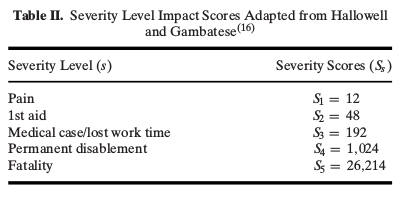
\includegraphics[width=300px]{table_severite}
\end{frame}

\begin{frame}
	On a maintenant la matrice creuse RP , \\
	\begin{tabular}[t]{lcccc}
		rapport & $w_1$ & $w_2$ & ... & $w_{80}$ \\
		$\textrm{rapport}_1$ & 1 & 0 &  & 1 \\
		$\textrm{rapport}_2$ & 1 & 0 &  & 1 \\
		$\textrm{rapport}_3$ & 0 & 1 &  & 1 \\
		... &  &  &  & \\
		$\textrm{rapport}_{814}$ & 1 & 1 &  & 1 \\
	\end{tabular}\\ 
	\bigskip
	et une table de vérité \\
	\begin{tabular}[t]{lc}
		rapport & sévérité  \\
		$\textrm{rapport}_1$ & $s_1$ \\
		$\textrm{rapport}_2$ & $s_2$ \\
		$\textrm{rapport}_3$ & $s_3$ \\
		... &  \\
		$\textrm{rapport}_{814}$ & $s_{814}$ \\
	\end{tabular}
\end{frame}

\begin{frame}
	Les auteurs ont fait une estimation de la valeur du risque $R_p$ pour chaque précurseur de la façon suivante\\
	$$R_p = \sum_{s=1}^{5} (n_{ps}S_s) $$
	avec $n_{ps}$ égal au nombre d'incident ayant une sévérité S le précurseur p est associé, et $S_s$ la valeur numérique du risque tel que vu à la Table II.\\
	\bigskip
	Les auteurs ont aussi corrigé les risques des précurseurs pour leur fréquece d'exposition.
	$$RR_p = \frac{1}{e_p} R_p$$
	avec $e_p$ la fréquence relative d'exposition d'un certain précurseur.
\end{frame}

\begin{frame}
	Petite note, l'article semble avoir une erreur concernant cette formule. Les codes R fournis par Trexier font une moyenne telle que 
	$$R_p = \frac{\sum_{s=1}^{5} (n_{ps}S_s)}{N}  $$
	avec $n_{ps}$ égal au nombre d'incident ayant une sévérité S le précurseur p est associé, $S_s$ la valeur numérique du risque tel que vu à la Table II, et N le nombre total de rapport analysés (N=814).\\
\end{frame}

\begin{frame}
	Maintenant que le risque par précurseur est déterminé, il est possible de recalculer le risque par rapport 
	$$R_{rapport_t} = \sum_{p=1}^{P} RR_p * \delta_{rp}$$
	avec $\delta_{rp}$ = 1 si le précurseur est présent dans le rapport et 0 autrement.
\end{frame}

\begin{frame}
	Autre petite note, faisons l'hypothèse que tous les précurseurs sont identiquement probable sur le chantier, de telle sorte que $e_p = 1, \forall p$ et ainsi que $RR_p = R_p$. \\
	\bigskip
	Il est ainsi possible de calculer l'erreur quadratique moyenne sur 
	$$\widehat{R_{rapport_t}} = \sum_{p=1}^{P} R_p * \delta_{rp}$$
	en comparant cette valeur avec $s_{rapport_t}$\\
	\bigskip
	Essaie de technique de régression en apprentissage automatique. Les modèles de séparateur a vaste marge (SVM), forêt aléatoire et régression linéaire seront comparées (train 85\%, test 15\%).
\end{frame}

\begin{frame}[c]
	Comparaison des erreur de régression 
	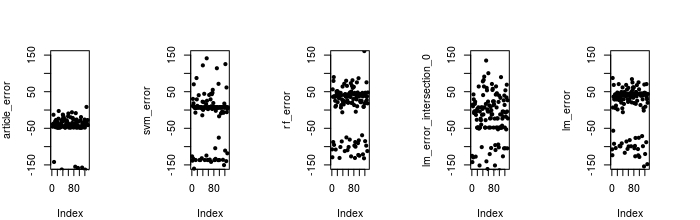
\includegraphics[width=330px] {error_comparison}
\end{frame}


\begin{frame}
	\textbf{Comparaison des erreur quadratiques moyennes}
	\begin{itemize}
		\item Méthode article: 1015
		\item SVM: 753
		\item Forêt aléatoires: 726
		\item Régression linéaire, intersection à 0: 794
		\item Régression linéaire: 710 
	\end{itemize}

	Il semble clairement y avoir un possibilité d'amélioration. Il faudrait réfléchir comment intégrer les poids des probabilité de trouver un précurseur sur le chantier. Est-ce qu'une nouvelle méthode de pondération (TFIDF / BNS) serait pertinente?
\end{frame}


\begin{frame}[t]
	Avec les $R_{rapport_t}$ calculés tel que dans l'article, \\
	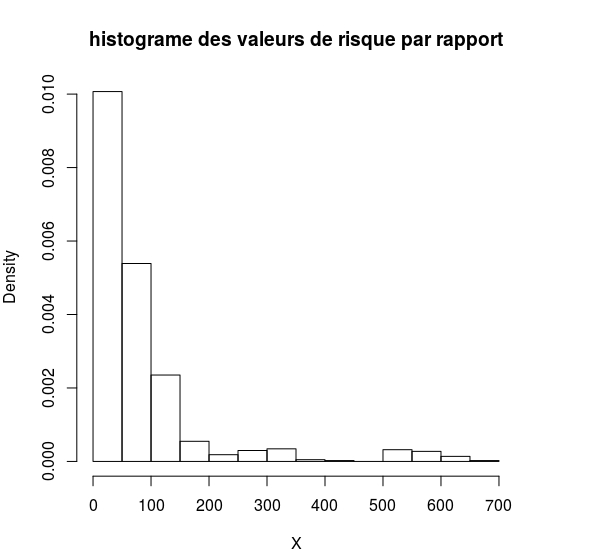
\includegraphics[height=200px] {histogramme_par_rapport}
	
\end{frame}


\begin{frame}[t]
	
	Modélisation de la fonction de densité
	\begin{itemize}
	\item Utilisation de noyaux pour estimer la densité (KDE) - pas EVT
\end{itemize}

Estimation par noyaux 

\begin{itemize}
	\item $\widehat{f(x)} = \frac{1}{nh} \sum^{n}_{i=1}K\big{(} \frac{x-x_i}{h},h \big{)}$
	\item choix d'un noyau N(0,1), avec fonction de densité $\frac{1}{\sqrt{2\pi}}e^{-x^2/2}$
	\item $\widehat{f(x)} = \frac{1}{n(2h^2\pi)^{p/2}}\sum^{n}_{i=1}e^{\frac{-1}{2}\big{(}\frac{x_{i}-x}{h}\big{)}^2}$
	\item choix de $h = \frac{0.9 \textrm{min}(\sigma^2, \frac{Q_3-Q_1}{1.34})}{n^{1/5}}$
\end{itemize}


Simulation pour enrichir la fonction de densité

\begin{itemize}
	\item Utilisation d'une méthode de bootstrap lissée
	\item Algorithme pour j simulation prenant R rapports en entrée:
		\begin{enumerate}		
		\item choisir un nombre entre 1 et R 
		\item tirer alétoirement $\epsilon_j$ avec $\epsilon_j \sim N(0,h_{x^2})$ 		
		\item créer une observation $X_{sim_j} = \bar{[X]} + \frac{X_i - \bar{[X]} + \epsilon_j}{\sqrt{1+h_{x^2}/\hat{\sigma}^2_X}} 	$
		\end{enumerate}
	
\end{itemize}

\end{frame}



\begin{frame}[t]
	Avec les $R_{rapport_t}$ et $\widehat{f(x)}$ calculés tel que dans l'article, \\
	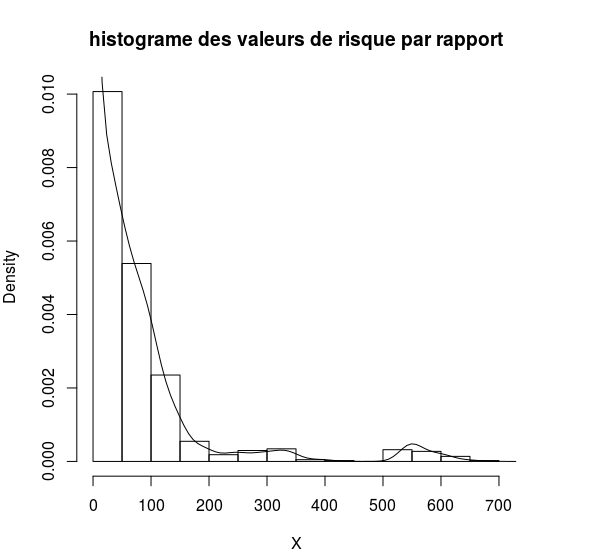
\includegraphics[height=200px] {histogramme_risque_rapport_kde}	
\end{frame}


\begin{frame}[t]
	Avec les $R_{rapport_t}$ et $\widehat{f(x)}$ calculés tel que dans l'article, \\
	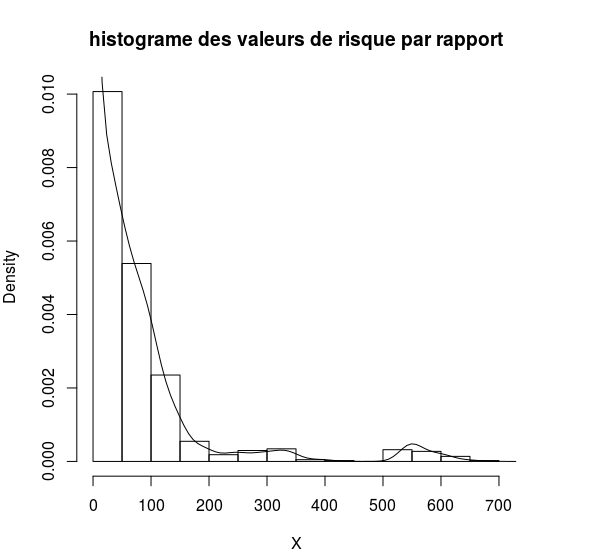
\includegraphics[height=200px] {histogramme_risque_rapport_kde}	
\end{frame}




